%%%%%%%%%%%%%%%%%%%%%%%%%%%%%%%%%%%%%%%%%%%%%%%%%%%%%%%%%%%%
%%% ELIFE ARTICLE TEMPLATE
%%%%%%%%%%%%%%%%%%%%%%%%%%%%%%%%%%%%%%%%%%%%%%%%%%%%%%%%%%%%
%%% PREAMBLE 
\documentclass[9pt,lineno]{elife}
% Use the onehalfspacing option for 1.5 line spacing
% Use the doublespacing option for 2.0 line spacing
% Please note that these options may affect formatting.
% Additionally, the use of the \newcommand function should be limited.


\usepackage{lipsum} % Required to insert dummy text
\usepackage[version=4]{mhchem}
\usepackage{siunitx}
\DeclareSIUnit\Molar{M}

% \makeglossaries

\newglossaryentry{n}{
    name=\ensuremath{n},
    description={target site}
}

%%%%%%%%%%%%%%%%%%%%%%%%%%%%%%%%%%%%%%%%%%%%%%%%%%%%%%%%%%%%
%%% ARTICLE SETUP
%%%%%%%%%%%%%%%%%%%%%%%%%%%%%%%%%%%%%%%%%%%%%%%%%%%%%%%%%%%%
\title{Bayesian analysis of the colocalization single molecule image data}

\author[1*]{Yerdos A. Ordabayev}
\author[1,2\authfn{1}\authfn{3}]{Larry Friedman}
\author[2\authfn{1}\authfn{4}]{Douglas Theobald}
\author[2*]{Jeff Gelles}
\affil[1]{Brandeis University}
\affil[2]{Institution 2}

\corr{email1@example.com}{FMS}
\corr{email2@example.com}{FS}

\contrib[\authfn{1}]{These authors contributed equally to this work}
\contrib[\authfn{2}]{These authors also contributed equally to this work}

\presentadd[\authfn{3}]{Department, Institute, Country}
\presentadd[\authfn{4}]{Department, Institute, Country}
% \presentadd[\authfn{5}]{eLife Sciences editorial Office, eLife Sciences, Cambridge, United Kingdom}


%%%%%%%%%%%%%%%%%%%%%%%%%%%%%%%%%%%%%%%%%%%%%%%%%%%%%%%%%%%%
%%% ARTICLE START
%%%%%%%%%%%%%%%%%%%%%%%%%%%%%%%%%%%%%%%%%%%%%%%%%%%%%%%%%%%%

\begin{document}

\maketitle

\begin{abstract}
Please provide an abstract of no more than 150 words. Your abstract should explain the main contributions of your article, and should not contain any material that is not included in the main text.
\end{abstract}


\section{Introduction}

Single-molecule fluorescence microscopy multi-wavelength colocalization methods (CoSMoS) are an important method for elucidating the mechanisms of complex biochemical processes \textit{in vitro}. CoSMoS is extensively used by labs that specialize in the technique and is increasingly being adopted by non-specialist labs as well. With the availability of good commercial microscopes, data analysis methodology is the major challenge in adoption and use of the CoSMoS technique.

Analysis of CoSMoS data is an intrinsically challenging problem. Although CoSMoS images are conceptually simple -- they consist only of diffraction-limited fluorescent spots collected in several wavelength channels -- efficient analysis of the images, reliable extraction of kinetic data, and fitting to model biochemical mechanisms are inherently challenging for several reasons. First, the number of photons emitted by a single fluorophore is limited by fluorophore photobleaching. Consequently, in many CoSMoS experiments one must work at the lowest feasible excitation power in order to maximize the duration of experimental recordings and to capture relevant kinetics. Achieving higher time resolution divides the number of emitted photons between a larger number of images. The required high concentrations of fluorescently tagged molecules create significant background noise \citep{peng_breaking_nodate, van_oijen_single-molecule_2011}, even with zero-mode waveguide instruments \citep{chen_high-throughput_2014}. These technical difficulties result in CoSMoS images that frequently have low signal-to-noise (S/N) ratios, making discrimination of real fluorescent spots from noise a major challenge. Second, there are transient non-specific interactions of the binder molecule with the surface of the microscope slide. These can result both in false positive colocalization detection when the binder molecule randomly lands near the target molecule and false negative detection when non-specific binding overlaps with the binder molecule at the target location by deforming its shape. These leads to erroneous estimates of the kinetic parameters and can be accounted for by joint analysis of the negative control locations and explicit modeling of non-specifically bound spots. Third, the kinetic analysis of thermally driven single molecule reactions is inherently statistical. Even if image analysis is perfectly reliable, statistical bias in the underlying experimental data (e.g., under-counting short binding events) can lead to erroneous mechanistic conclusions. In real experiments, where image analysis is necessarily less than perfect, there is a need to quantitatively account for the uncertainties in CoSMoS image data to deduce molecular mechanisms.

Current spot detection methods are based on extracting quantitative features of the spot (e.g., intensity profile, size, shape, and distance to target) from the 2-D image and then identifying spots using manually chosen thresholds for these parameters \citep{friedman_cosmos_analysis_2015, smith_automated_2019}. These image analysis based methods are more accurate than previous approaches in part because they make use of information contained in the 2-D images that are disregarded when only the integrated intensity is used \citep{friedman_cosmos_analysis_2015}. While these methods greatly improve CoSMoS data analysis, they nevertheless suffer from significant deficiencies. First, current methods require subjective choice of user-set thresholds for spot amplitude, diameter and proximity. These settings significantly affect error rates and no objective method to select them currently exists, making the approach non-robust and overly complicated. Second, it is unsatisfying that existing analysis methods are discontinuous and there is a loss of information at each step of the analysis. Image classification is performed on extracted features of the spot and not the raw 2-D images themselves. Furthermore, image classification step produces only a binary output (spot present or absent); they do not output the probability of spot presence in marginal images, a critical feature in the analysis of low S/N data. Kinetic analysis, in turn, is based on the binary output of the image classification step further reducing the amount of information transmitted from the raw images. Third, it is nontrivial to incorporate prior knowledge (e.g., colocalization accuracy, size of the spot, frequency of non-specific binding) into these analysis methods.

Here we present novel, objective, statistically based approach for analysis and interpretation of CoSMoS data. Our new method: 1) maximizes extraction of useful results from data (particularly at the low S/N inherent to many CoSMoS experiments) by analyzing raw images, not just fluorescence intensities; 2) applies single global probabilistic model which allows to directly infer model parameters from CoSMoS image data and priors; 3) explicitly models non-specific interaction of the binder molecule with the surface which allows to jointly analyze negative control dataset; 4) uses Gamma distribution as a more realistic intensity noise model rather than Gaussian distribution; 4) has a flexible framework that can naturally be extended to kinetic models and multi-wavelength analysis. Our new analysis method will increase the accessibility of the CoSMoS method to investigators that have important biological problems to solve but are not able to develop their own data analysis methods or to reliably use the current data analysis approaches which require extensive parameter tweaking. The method developed here eliminates dependence on subjective parameter adjustments and include built-in tools for statistical assessment of the validity of the results as essential steps in the analysis process.

\begin{comment}
Coordinate optimization of CoSMoS image and mechanistic/kinetic models. We propose analyzing CoSMoS data using a novel approach in which we co-optimize inference of both CoSMoS image classifications and the underlying molecular kinetic mechanism simultaneously, by integrating the Bayesian image and kinetic analysis together under a single global probabilistic model. This approach is inspired by previously successful applications of Hidden Markov Models (HMMs) to elucidate kinetic mechanisms and derive realistic rate constants from scalar time series data (e.g., from smFRET and single-channel electrophysiology experiments such as in refs. 11–16). To our knowledge this approach has not previously been extended to inferring biochemical reaction mechanisms directly from 2-D single-molecule images.
 
The proposed research will facilitate the application of CoSMoS to more complex biological systems and experiments. As the CoSMoS technique has become better established, its applications have become increasingly complex. In some published and unpublished studies we now routinely work at labeled molecule concentrations approaching 1 µM, perform three- and four-color experiments, simultaneously analyze binding to multiple types of separately identified target molecules in the same microscope field of view, and examine in vitro systems of biochemical complexity up to and including whole cell extracts. Such complex experiments present increasingly difficult problems of data analysis. The proposed research (Aim 2) will greatly aid in the interpretation of the complex data sets produced by the current generation of CoSMoS experiments by integrating the capability to do the time series analyses and kinetic modeling needed for mechanistic interpretation of the data. They will allow accurate elucidation of complex molecular mechanisms and efficient accommodation of experimental imperfections like photobleaching and incomplete labeling.

Background: Differences between analysis of CoSMoS data and analysis of super-resolution or single-molecule tracking data. Super-resolution techniques like PALM and STORM45–47 are superficially similar to CoSMoS, as they also involve localizing spots of single-molecule fluorescence. The same is true for live-cell single-molecule fluorescence detection/tracking methods (e.g., refs. 48–51). However, these applications differ from CoSMoS in fundamental ways: 1) PALM and STORM use comparatively high S/N, short duration imaging to maximize the spatial precision of spot localization. CoSMoS is the opposite; much poorer spatial precision is needed but long duration recordings of individual molecules (with consequent lower S/N) are required to provide information about kinetic processes. 2) CoSMoS image analysis is predicated on making use of prior information about the surface locations of target molecules; no such prior information exists in super-resolution or tracking applications. 3) Unlike CoSMoS, neither super-resolution nor tracking experiments are directly tied to underlying biochemical kinetic reaction schemes. Thus, while there has been extensive development of analytical methods for super-resolution and tracking (including some use of Bayesian approaches7–10,52,53), optimal analysis of CoSMoS data will require specifically tailored methodology.

Preliminary results 3: 2-D image-based CoSMoS data analysis. (Ref. 6) The most basic task in CoSMoS data analysis is spot discrimination. The goal is to acquire information at each time point about whether a binder molecule fluorescence spot is observed at the image position of a target molecule (e.g., whether a co-localized green RNA polymerase is observed at the surface location of a blue DNA spot in Figure 1). The discrimination methods that are commonly used (including in earlier work from the Gelles lab26,29,36,38,57,59,60) involve some combination of purely subjective inspection of the microscope images and an objective method based on integrating the binder fluorescence intensity over small regions of the image (typically squares ~0.4 μm on a side) centered on the location of the target molecule and then using crossings of set intensity threshold(s) to score binder molecule arrival and departure. For reasons described in detail elsewhere6 , these approaches are both imprecise and inaccurate, particularly when applied to the low S/N images often used. A fundamental problem with these methods is that even their objective and quantitative components rely on the integrated intensity and thus discard spatial information contained in the images that can and should be used to objectively inform decisions about spot presence.
\end{comment}

%\section{Results}

\subsection{The Model}

In this work, we present a probabilistic generative model for single-molecule image-data and describe Bayesian inference approach used to obtain posterior distributions of latent model parameters. The generative model can be interpreted as a causal process that produces the observed image data. The graphical model in Figure 2A visually describes latent variables of the model and conditional independence structure of the model. We model the observed image as ``spot'' images of binder molecules superimposed on background image. Fluorescence spots are modeled as a 2D Gaussians parameterized by a set of variables ($h, w, x, y$) which accurately approximates fluorescence microscope point spread function \cite{Zhang2007-rb}. The model depends on various unobserved physical parameters such as background photon intensity and the number, position, shape, and intensity of each spot in the image. The unobserved parameters, in turn, are described by prior distributions which embed into the model our existing knowledge of the experiment, such as the likely position of an on-target spot. Explicitly model on-target and off-target spots.

Our model assumes that at maximum 2 spots in total can be present in a single image and at maximum only one on-target spot. The image model described above allows to capture many of the characteristics of real experimental data, such as site and time dependent fluctuations in the local background signal, time dependent fluctuations in the spot intensity and its position, simultaneous binding of on-target and off-target spots, Gamma distributed noise, which is more realistic than Gaussian noise. Figure 2B,C,D shows examples where there is no spot, one spot, or two spots and corresponding spot parameters in the table.

Total observed intensity is the sum of the offset signal (dark current) plus the photon counts amplified by the gain setting of the camera. The linear relationship between the noise variance and the mean intensity is built into the intensity model through the gain and offset parameters and the gain parameter is fitted along with other parameters. Distribution of the offset signal is obtained as a histogram density signal from the single-molecule images (Figure ).  In Figure we show raw images and their intensity distributions along with the images simulated from the posterior distribution (posterior predictive checking). Comparison of images and distributions for spot/no spot cases show that our model accurately models intensity as a function of mean intensity reflecting the dependence of the noise on the mean intensity. Additionally, Figure shows that the gain parameter is accurately inferred for a simulated set of data with varying gain parameter where the true value of the gain parameter is known.

\subsection{Bayesian Inference and Implementation}

Posterior distributions of latent variables conditioned on the observed data is given by the Bayes' theorem. The evidence in general is intractable. Here we use stochastic variational inference (SVI) approach and maximize the evidence-lower bound (ELBO). Our program Tapqir is open-source (github link) and is implemented in the probabilistic programming language Pyro. The advantage of using PPL like Pyro is its black box SVI approach which allows to focus on the model, efficient computation on GPU, scalability to large datasets. Details of the generative model and variational model are given in the online Methods section.

\subsection{Analysis of simulated data}

As a validation of our model we demonstrate its application to simulated synthetic data. Fake-data simulation is important because it allows to directly check that the inference on latent variables is reliable. Thus, fake-data simulation provides an upper bound of what can be learned reliably about the model for various types of data. Simulation parameters details are described in the online Methods. We made 10 randomized simulations and then fit the synthetic data to the model. Figure 3 shows plots of the simulated values of the global parameters (gain, average on-target spot probability, average off-target spot probability, proximity) vs the fitted values. The results demonstrate that model parameters can be reliably recovered which is good.

MCC plot. Example traces.

\subsection{Analysis of experimental data}

Thermodynamic Analysis.

In this section, we describe different aspects of our model. The Bayesian model described here is holistic in a sense that the observed data and all of the model parameters are interconnected. However, its modular structure allows to view and analyze different parts of the model separately. Below we review briefly the CoSMoS method and the type of data generated by CoSMoS experiments, and then describe the image model, the intensity model, spot-detection, and co-localization aspects of the model.

\subsection{Multi-wavelength single-molecule co-localization methods}

Before describing the approach used for the analysis of CoSMoS data, it is helpful to  review briefly the experimental method. The key features of a CoSMoS experiment include: 1) One species of fluorescently labeled molecule (called the “target”) is tethered to the surface of the observation chamber. Target molecules are immobilized at a surface density sufficiently low that the mean nearest-neighbor distance is large relative to the point-spread function (i.e., the diffraction-limited spot size) of the microscope. 2) Molecules, each species labeled with a different dye color, are added to the solution over the surface, typically at concentrations $\leq 1 \mu$M. When these “binder” molecules are freely diffusing in solution, they are invisible in TIRF. In contrast, when they are bound to the target, single binder molecules are detected as discrete fluorescent spots (Figure \ref{fig:cosmos_experiment}). The combination of features 1 and 2 means that formation of an individual binder-target complex is detected as spot appearance; dissociation of a binder-target complex is detected as spot disappearance \cite{Friedman2006-kb, Friedman2015-nx}.

\subsection{CoSMoS image data}

CoSMoS data analysis requires identifying the locations of target molecules and the corresponding positions in the binder molecule camera channel. Image pre-processing steps include alignment of images from multiple wavelength channels and drift correction \cite{Friedman2015-nx, Smith2019-yb}. Single-molecule images after pre-processing steps consists of a $P \times P$ matrix of pixel intensities with the target molecule at the center of the image. One experiment typically consists of a set of images where we have $N$ target sites ($n \in \{1,\dots,N\}$) each consisting of a series of $F$ different images in a recording ($f \in \{1,\dots,F\}$) (a “recording”).

CoSMoS images consist of offset signal, background intensity and diffraction-limited spots. Detection of on-target binding depends on the intensity of the spot and its distance to the target molecule. The size $P=14$ of the selected area is chosen to be large enough to detect the on-target spot and reliably determine the local background intensity. In addition to the on-target spot, non-specifically bound binder molecules can also be present in the image. Usually no more than two spots are present in the single image. Frequently, identification of on-target binding is complicated by molecules binding off-target which distort the shape of the on-target spot and its apparent distance to the target. 

%\begin{figure}
%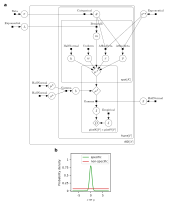
\includegraphics[width=\linewidth]{figures/figure1.jpg}
%\caption{Co-localization single molecule spectroscopy experiment. (A) Target molecules are localized in the blue channel and then on-target and off-target areas of interest are selected. (B) Movies of the binder molecule collected in the green channel. In selected AoI binder molecules can be on-target, off-target, or absent.}
%\label{fig:cosmos_experiment}
%% If the optional argument in the square brackets is "none", then the caption *will not appear in the main figure at all* and only the full caption will appear under the supplementary figure at the end of the manuscript.
%\figsupp[Shorter caption for main text.]{This is a supplementary figure's full caption, which will be used at the end of the manuscript.}{\includegraphics[width=6cm]{frog}}\label{figsupp:sf1}
%\figsupp{This is another supplementary figure.}{\includegraphics[width=6cm]{frog}}
%\figdata{This is a description of a data source.}\label{figdata:first}
%\figdata{This is another description of a data source.}\label{figdata:second}
%\end{figure}

%\begin{figure}
%\includegraphics[width=\linewidth]{figures/figure3a.png}
%\includegraphics[width=\linewidth]{figures/figure3b.png}
%\includegraphics[width=\linewidth]{figures/figure3c.png}
%\caption{Co-localization single molecule spectroscopy experiment. (A) Target molecules are localized in the blue channel and then on-target and off-target areas of interest are selected. (B) Movies of the binder molecule collected in the green channel. In selected AoI binder molecules can be on-target, off-target, or absent.}
%\label{fig:view}
%\end{figure}

\subsection{Image Model Module} 

We model the observed image as ``spot'' images of binder molecules superimposed on background image. In particular, background image consists only of constant background intensity $\mathrm{b}_{nf}$ that can vary from image to image. Our model assumes that at maximum $K=2$ number of spots can be present in a single image.  Fluorescence spot is modeled as a 2D Gaussian which accurately approximates fluorescence microscope point spread function \cite{Zhang2007-rb}. Each spot is parameterized by integrated scalar intensity $\mathrm{h}_{nfk}$, width $\mathrm{w}_{nfk}$, and relative position $\mathrm{x}_{nfk}$ and $\mathrm{y}_{nfk}$ to the target molecule. All of the spot parameters are local/individual for each spot.

We use binary indicator variable $\mathbf{m} = \{\mathrm{m}_{nfk}\}$ to denote the presence of each individual spot ($k \in \{1,\dots,K\}$). The value of the index variable $\theta_{nf} \in \{0,1,\dots,K\}$ specifies the index of the on-target spot when it is present and equals zero when the on-target spot is absent. There are $2^K + K2^{K-1}$ unique combinations of $\mathrm{m}$ and $\theta$ which define the state space for each image. Table~\ref{tab:states} shows the state space when $K=2$. Thus, we get the image model ($\mu^I_{nfij}$) calculated as the sum of the background intensity ($\mathrm{b}_{nf}$) and 2D Gaussian spots ($\mu^S_{knfij}$) present in the image.

\subsection{Spot Detection}

WIP

Spot detection is performed in a probabilistic manner. Spot existence probability depends on the information in the entire image. However, it primarily correlates with the intensity of the spot. Discrimination of spots from random fluctuations in the background signal depends on the prior and not on the threshold parameter. In the absence of prior information uninformative prior can be used. Plotting results show that with half normal prior spots have to be roughly above 1 SNR.

\subsection{Co-localization}

For the spots that are present in the image they can be further classified as on-target (co-localization) or off-target (non-specific). The probability of being on-target or off-target is dictated primarily by the distance to the target. Spots bound on-target and off-target have different prior distributions of their location relative to the target molecule. This prior knowledge is used to discriminate between on- and off-target spots in a probabilistic manner using mixture distributions model. Off-target spots have a uniform prior distribution across the image and can bind anywhere on the surface with equal probability. On-target spots, on the other hand, are clustered near the target molecule. Standard deviation of the distribution of on-target spots depends on the spot localization accuracy and the mapping accuracy between target and binder channels (?). By analyzing simulated data we have established that this parameter, also called the proximity parameter, can be reliably determined by floating it during the fit (Figure ). Alternatively, proximity parameter can be determined experimentally and fixed in the model. Figure show the distribution of the center of mass of on-target spots which are tightly clustered around the target molecule. On the other hand, off-target spots are distributed more uniformly across the area of the image.

Second, the posterior probabilities of being classified as on-target or off-target spot depends on the prior average frequencies of on-target and off-target spots. Increasing the ratio of the off-target molecules to on-target molecules decreases the probability of the spot being on-target reflecting the fact that.

This standard distribution can be determined independently and used as a fixed parameter in the model. However, it can also be floated in the fit and determined from the overall distribution of the center of masses of spots. $\sigma^{xy}$, $\pi^z$, and $\lambda^j$ are correlated. Figure shows simulated data with varying parameters where the true values of parameters are inferred correctly. Note that the posterior probability of the spot class depends on its relative position to the target and average probabilities of on-target and off-target spots.

\subsection{Informal Kinetic/Thermodynamic Analysis}

WIP

%\section{Discussion}

\lipsum[9]

%\section{Methods}

\begin{comment}
\subsection{Approach}

\subsubsection{Probabilistic modeling based on fundamental statistical analysis of data and priors}

To solve the problems with existing CoSMoS data analysis methods identified above, we have developed a new image-analysis-based approach that is accurate, objective, and built on a rigorous statistical approach to the CoSMoS image analysis problem. This method is based on probabilistic modeling methodology. Bayesian model is a statistical model where probability is used to represent all uncertainty within the model, both for observed and hidden quantities in a system of interest. Bayes' theorem allows to perform inference on hidden variables given the observed data. The method described here is time-independent meaning that we ignore the time dimension of the recording -- the order of the images is arbitrary and does not affect the model, as each image is considered statistically independent of the others. We note that this time-independent method can naturally be extended into a time-dependent approach to both more accurately analyze the images and to directly obtain information about molecular kinetic mechanisms.  The proposed methods will eliminate the need for subjective image inspection and minimize the manual work required for CoSMoS data analysis. 

Unlike standard analysis methods for CoSMoS and single molecule FRET (smFRET), which are based on scalar intensity measurements derived from integration of emission in image regions of interest, our model fully uses information contained in the raw two-dimensional microscope images. The value of image data is proven in previous studies \citep{Friedman2015-nx,Smith2019-yb}. To analyze the CoSMoS image classification problem within a Bayesian framework, one must define ideal image shapes for each class (image model) and choose a likelihood function for the observed data (noise model).
\end{comment}

The images are diffraction-limited point spread functions. CoSMoS images consist of background intensity and diffraction-limited spots. The CoSMoS data set consists of a set of images where we have $N$ target sites ($n \in \{1,\dots,N\}$) each consisting of a series of $F$ different images in a recording ($f \in \{1,\dots,F\}$) (a “recording”). Each image is represented as a matrix (2D-array) of $P \times P$ pixel intensities ($i,j \in \{1,\dots,P\}$). We denote entire data set as a multi-dimensional array $D$ and the value of a specific pixel intensity as $D_{nfij}$.

Our goal is to extract useful information from the data such as the probability of the presence of the on-target molecule. Our approach is to use statistical modeling. We formulate a generative model that describes how the observed data is produced. Then we make inference on latent variables that describe the physical parameters of the generative model. 

\subsection{Model}

We build a probabilistic model for CoSMoS data by introducing latent variables that explain how the observed data is generated. A graphical model describing the probabilistic relationships in the model is shown in Figure \ref{fig:graph}. In this directed graph, nodes are either random variables (circles) or deterministic functions (diamonds). Related nodes are connected by edges, with an arrow pointing towards the dependent variable. Dashed boxes represent activation of variables. Finally, plates represent replication and specify an index for the repeated variable.

\begin{figure}[ht]
  \begin{center}
    % model_pca2.tex
%
% Copyright (C) 2010,2011 Laura Dietz
% Copyright (C) 2012 Jaakko Luttinen
%
% The MIT License
%
% See LICENSE file for more details.

% PCA model

%\beginpgfgraphicnamed{model-pca}
\begin{tikzpicture}

  % Define nodes

  % Y
  \node[obs]          (D)   {$D$}; %

  % W and X
  \node[det, above=of D]            (md) {$\mu^D$} ; % 
  \node[latent, above=of md] (w)   {$w$}; %
  \node[latent, above=of md, left=of w]  (h)   {$h$}; %
  \node[latent, above=of md, left=of h]  (b)   {$b$}; %
  \node[latent, above=of md, right=of w]  (x)   {$x$}; %
  \node[latent, above=of md, right=of x] (y)   {$y$}; %

  % b hyperparameters
  \node[const, above=2.8 of b, xshift=-0.5cm] (mb) {$\mu^b$} ; %
  \node[const, above=3.5 of b, xshift=0.5cm]  (bb) {$\beta^b$} ; %

  % h hyperparameters
  \node[const, above=3.5 of h, xshift=-0.5cm] (mh) {$\mu^h$} ; %
  \node[const, above=3.5 of h, xshift=0.5cm]  (bh) {$\beta^h$} ; %

  % w hyperparameters
  \node[const, above=3.5 of w, xshift=-0.5cm] (mw) {$\mu^w$} ; %
  \node[const, above=3.5 of w, xshift=0.5cm]  (nw) {$\nu^w$} ; %

  % xy hyperparameters
  \node[const, above=3.5 of x, xshift=-0.1cm] (mxy) {$\mu^{x,y}=0$} ; %
  \node[const, above=3.5 of y, xshift=0.1cm] (pr) {$(2,proximity)$} ; %
  \node[det, above=1.4 of y]  (nxy) {$\nu^{x,y}$} ; %

  % Factors
  \factor[above=of D] {D-f} {left:$\mathcal{G}$} {} {} ; %
  \factor[above=0.6 of b] {b-f} {left:$\mathcal{G}$} {mb,bb} {b} ; %
  \factor[above=0.6 of h] {h-f} {left:$\mathcal{G}$} {mh,bh} {h} ; %
  \factor[above=0.6 of w] {w-f} {left:$\mathcal{B}$} {mw,nw} {w} ; %
  \factor[above=0.6 of x] {x-f} {left:$\mathcal{B}$} {mxy,nxy} {x} ; %
  \factor[above=0.6 of y] {y-f} {left:$\mathcal{B}$} {mxy,nxy} {y} ; %

  % D hyperparameters
  \node[const, right=8 of D-f] (g) {gain} ; %

  % m and theta
  \node[latent, right=of y-f] (m)   {$m$}; %
  \node[latent, above=0.5 of m] (t)   {$\theta$}; %

  % m and theta hyperparameters
  \node[det, right=1. of m]        (pm) {$\pi^m$} ; %
  \node[det, right=1. of t]        (pt) {$\pi^\theta$} ; %
  \node[const, right=of pt] (pz) {$\pi^z$} ; %
  \node[const, right=of pm] (lj) {$\lambda^j$} ; %

  % theta hyperparameters
  %\node[const, right=1.2 of t] (pt) {$\pi^\theta(\pi^z,\lambda^j)$} ; %

  % noise
  %\node[latent, right=2.5cm of y-f]         (t)   {$\tau$}; %
  %\node[const, above=of t, xshift=-0.5cm] (at)  {$\alpha_\tau$} ; %
  %\node[const, above=of t, xshift=0.5cm]  (bt)  {$\beta_\tau$} ; %

  % Factors
  \factor[right=of m] {m-f} {above:$\mathcal{C}$} {pm} {m} ; %
  \factor[right=of t] {t-f} {above:$\mathcal{C}$} {pt} {t} ; %
  %\factor[above=of x] {x-f} {left:$\mathcal{N}$} {mx,ax} {x} ; %
  %\factor[above=of t] {t-f} {left:$\mathcal{G}$} {at,bt} {t} ; %
  %\factoredge {dot,t} {y-f} {y} ; %

  \gate {m-gate} {(h-f)(h-f-caption)(h-f)(h-f-caption)(w-f)(w-f-caption)(x-f)(x-f-caption)(y-f)(y-f-caption)} {m}

  % Connect w and x to the dot node
  \factoredge[-] {g,md} {D-f} {D} ;
  \edge[-] {b,h,w,x,y} {md} ;
  \edge[-] {pz,lj,m} {pt} ;
  \edge[-] {pz,lj} {pm} ;
  \edge[-] {t,pr} {nxy} ;

  % Plates
  \plate {K} { %
    (h)(h-f)(h-f-caption) %
    (w)(w-f)(w-f-caption) %
    (x)(x-f)(x-f-caption) %
    (y)(y-f)(y-f-caption) %
    (m-gate) %
    (nxy)
  } {$\forall k \in \{ 1..K \}$} ;
  \plate {F} { %
    (K)
    (t)(t-f)(t-f-caption)(pt) %
    (m)(m-f)(m-f-caption)(pm) %
    (b)(b-f)(b-f-caption) %
    (md) %
    (D)(D-f)(D-f-caption) %
  } {$\forall f \in \{ 1..F \}$} ;
  \plate {N} { %
    (F)
    (mb)
  } {$\forall n \in \{ 1..N \}$} ;
  %\plate {} {%
    %(y)(y-f)(y-f-caption) %
    %(w)(w-f)(w-f-caption) %
    %(dot) %
    %(yx.north west)(yx.south west) %
  %} {$M$} ;

\end{tikzpicture}
%\endpgfgraphicnamed

%%% Local Variables: 
%%% mode: tex-pdf
%%% TeX-master: "example"
%%% End: 


  \end{center}
  \caption{Graphical model for the Bayesian classification model used in Pyro. The model has a modular structure consisting of three parts: classifier, the spot model, and the noise model. Hidden variables (circles) - background intensity ($b$), integrated intensity of the spot ($h$), width of the spot ($w$), position of the spot on the $x$-axis ($x$) and on the $y$-axis ($y$), existence indicator of spots ($m$), and index of the on-target spot ($\theta$). Observed variable (shaded circle) - image of the area of interest ($D$). Variables nested in plates are repeated for a number of times displayed at the bottom-right corner - target sites ($N$), frame count ($F$), number of spots in a single image ($K$). Densities are depicted as  small filled boxes. Deterministic functions are depicted as diamonds. Constants and hyperparameters are written without any borders. Gate (dashed box) represents variable activation conditioned on another variable.}
  \label{fig:graph}
\end{figure}

\subsubsection{Physical model}

We model the observed image data as ``spot'' images of binder molecules superimposed on background image. In particular, background image consists only of constant background intensity $\mathrm{b}_{nf}$ that can vary from image to image. Our model assumes that at maximum $K$ number of spots can be present in a single image.  Fluorescence spot is modeled as a 2D Gaussian which accurately approximates fluorescence microscope point spread function \citep{Zhang2007-rb}. Each spot is parameterized by integrated scalar intensity $\mathrm{h}_{nfk}$, width $\mathrm{w}_{nfk}$, and positions $\mathrm{x}_{nfk}$ and $\mathrm{y}_{nfk}$ on the image:

\begin{equation}
    \mu^{S}_{nfkij} =
        \dfrac{\mathrm{h}_{nfk}}{2 \pi \mathrm{w}^2_{nfk}} \exp{\left[ -\dfrac{(i-\mathbf{x}_{nfk})^2 + (j-\mathrm{y}_{nfk})^2}{2\mathrm{w}^2_{nfk}} \right]}
\end{equation}

We use binary indicator variable $\mathbf{m} = \{\mathrm{m}_{nfk}\}$ to denote the presence of each individual spot ($k \in \{1,\dots,K\}$). The value of the index variable $\theta_{nf} \in \{0,1,\dots,K\}$ specifies the index of the on-target spot when it is present and equals zero when the on-target spot is absent. There are $2^K + K2^{K-1}$ unique combinations of $\mathrm{m}$ and $\theta$ which define the state space for each image. Table~\ref{tab:states} shows the state space when $K=2$.

Thus, we get the image model ($\mu^I_{nfij}$) calculated as the sum of the background intensity ($\mathrm{b}_{nf}$) and 2D Gaussian spots ($\mu^S_{knfij}$) present in the image:

\begin{equation}
    \mu^\mathrm{I}_{nfij} = \mathrm{b}_{nf} + \sum_{\mathrm{m}_{nfk}=1} \mu^S_{knfij}
\end{equation}

\begin{figure}
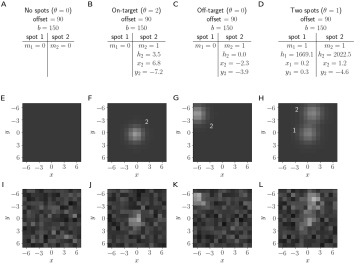
\includegraphics[width=\linewidth]{figures/figure2/figure2.png}
%\includegraphics[width=\linewidth]{figures/figure2g.png}
\caption{Image models. CoSMoS images are modeled as 2D Gaussian spots superimposed onto the background intensity and the offset. Examples of the ideal image shapes for cases when there are (A,E,I) no spots, (B,F,J) single on-target spot, (C,G,K) single off-target spot, and (D,H,L) two spots. Noisy images (I-L) are generated using Gamma distribution with the parameter gain = 7 as described in the text.}
\label{fig:model}
\end{figure}

\subsubsection{Noise model}

\begin{comment}
Shot noise originates from a stochastic nature of photon counting which can be modeled by a Poisson process. The number of photons that fall on each pixel of the camera is Poisson distributed where the variance of the signal equals the mean value of the signal. Gain is a camera setting that amplifies the signal from camera sensors. Our model uses Gamma distribution parameterized by mean intensity ($\mu^D_{nfij}$) and gain ($g$) to model the linear relationship between the expected value of the signal and the variance with which the signal scatter about its expected value. Figure \ref{fig:model}  shows images  where the ideal images were perturbed with Gamma noise for no-spot (D), single spot (E), and two spots (F) images.
\end{comment}

Observed images are contaminated by noise. Noise is a stochastic phenomenon and therefore is described by the likelihood function. The likelihood describes the probability of the observed image given the image model. Scatter about the expected value of signal intensity ($\mu^I_{nfij}$) is determined by photon shot noise and the camera gain that amplifies the signal. We use Gamma distribution as a noise model which is more flexible than Gaussian noise and can better approximate Poissonian camera noise. In addition, there is a noise in the offset signal. Its distribution can be obtained from the camera images:

\begin{equation}
    I_{nfij} \sim \textbf{Gamma} (\mu^I_{nfij}, \sqrt{\mu^I_{nfij} \gamma})
\end{equation}

\begin{equation}
    \delta_{nfij} \sim \textbf{Categorical}_{\{ \delta_r \}^R_{r=1}}(\bm{\pi}^\delta)
\end{equation}

\begin{equation}
    D_{nfij} = \delta_{nfij} + I_{nfij}
\end{equation}

where $I_{nfij}$ is the signal intensity and $\gamma$ is the gain setting of the camera. $\delta_{nfij}$ is a camera offset and $\bm{\pi}^\delta$ is its distribution that can be obtained empirically from the dark corners of the images.

\subsubsection{Priors}
Prior distribution describe our assumptions about the model. On-target spots have a Bernoulli distribution with average probability $\pi^z$, while the number of off-target spots has a truncated Poisson distribution with the rate parameter $\lambda^j$. For the spot intensity we assume broad range of values given by:

\begin{equation}
    h_{knf} \sim \mathbf{HalfNormal}(\sigma^h)
\end{equation}
 
 Spot width has a uniform prior confined to a range:
 
\begin{equation}
    w_{knf} \sim \textbf{Uniform}(w_{\min}, w_{\max})
\end{equation}

Priors for the position of the spot depends whether the spot is on-target or non-specific. On-target spots are localized around the target molecule within the experimentally determined co-localization accuracy. On the other hand, non-specific binding can occur anywhere within the image and therefore has a uniform distribution across the image:

\begin{equation}
    x_{knf}, y_{knf} \sim
    \begin{cases}
    \textbf{AffineBeta}(0, \nu^{xy}, -\frac{P+1}{2}, \frac{P+1}{2}) & \text{$\theta_{nf} = k$ (on-target)} \\
    \textbf{Uniform}(-\frac{P+1}{2}, \frac{P+1}{2}) & \text{$\theta_{nf} \neq k$ (off-target)}
    \end{cases}
\end{equation}

Due to the irregularity of the filed of view of the microscope we assume separate prior for each target site:

\begin{equation}
    b_{nf} \sim \textbf{Gamma}(\mu^b_n, \sigma^b_n)
\end{equation}

\begin{table}
\caption{\label{tab:states}State space for $K = 2$.}
% Use "S" column identifier to align on decimal point 
\begin{tabular}{c c c c c}
\toprule
state   & first spot $m_{nf1}$ & second spot $m_{nf2}$ & on-target index $\theta_{nf}$  & probability \\
\midrule
$1$       & $0$     & $0$     & $0$         &  \\
$2$       & $1$     & $0$     & $0$         &  \\
$3$       & $0$     & $1$     & $0$         &  \\
$4$       & $1$     & $1$     & $0$         &  \\
$5$       & $\mathbf{1}$    & $0$     & $1$         &  \\
$6$       & $\mathbf{1}$    & $1$     & $1$         &  \\
$7$       & $0$     & $\mathbf{1}$    & $2$         &  \\
$8$       & $1$     & $\mathbf{1}$    & $2$         &  \\
\bottomrule
\end{tabular}
\end{table}

\subsubsection{Joint Distribution}

Factorization of the joint probability of the model is given by:

\begin{equation}
    p_\psi (\mathbf{D}, \mathbf{v})
    = p_\gamma (\mathbf{D} | \mathbf{b}, \mathbf{m}, \mathbf{h}, \mathbf{w}, \mathbf{x}, \mathbf{y})
    p_{\mu^b, \sigma^b} (\mathbf{b})
    p (\mathbf{h})^\mathbf{m}
    p (\mathbf{w})^\mathbf{m}
    p_{\sigma^{\mathrm{xy}}} (\mathbf{x}|\mathbf{\theta})^\mathbf{m}
    p_{\sigma^{\mathrm{xy}}} (\mathbf{y}|\mathbf{\theta})^\mathbf{m}
    p_{\pi^z, \lambda^j} (\mathbf{m}, \theta)
\end{equation} 

where $\psi = \{ \pi^z, \lambda^j, \mu^b, \sigma^b, \gamma \}$ and $\mathbf{v} = \{ \mathbf{b}, \mathbf{m}, \theta, \mathbf{h}, \mathbf{w}, \mathbf{x}, \mathbf{y} \}$.

\subsection{Inference}

The evidence, i.e. probability of the data, is given by:

\begin{equation}
    p_\psi (\mathbf{D}) = \int_\mathbf{v} p_\psi (\mathbf{D}, \mathbf{v}) d\mathbf{v}
\end{equation}

Our goal is to learn good model parameters by maximizing the log evidence:

\begin{equation}
    \psi_{\max} = \argmax_\psi \log p_\psi (\mathbf{D})
\end{equation}

In addition, we want to obtain the posterior over the latent variables $\mathbf{v}$ given the observed data:

\begin{equation}
    p_{\psi_{\max}} (\mathbf{b}, \mathbf{m}, \theta, \mathbf{h}, \mathbf{w}, \mathbf{x}, \mathbf{y}|\mathbf{D}) =
    \dfrac{p_{\psi_{\max}}(\mathbf{D}, \mathbf{b}, \mathbf{m}, \theta, \mathbf{h}, \mathbf{w}, \mathbf{x}, \mathbf{y})}
    {\int_{\mathbf{b}, \mathbf{h}, \mathbf{w}, \mathbf{x}, \mathbf{y}}
    \sum_{\mathbf{m}, \theta}
    p_{\psi_{\max}} (\mathbf{D}, \mathbf{b}, \mathbf{m}, \theta, \mathbf{h}, \mathbf{w}, \mathbf{x}, \mathbf{y})
    d\mathbf{b} d\mathbf{h} d\mathbf{w} d\mathbf{x} d\mathbf{y}}
\end{equation}

\begin{equation}
    p_{\psi_{\max}}(\mathbf{b}, \mathbf{m}, \theta, \mathbf{h}, \mathbf{w}, \mathbf{x}, \mathbf{y}|\mathbf{D})
    \simeq q_{\phi}(\mathbf{b}) q(\mathbf{m}, \theta) q(\mathbf{h})^\mathbf{m}
    q(\mathbf{w})^\mathbf{m} q(\mathbf{x})^\mathbf{m} q(\mathbf{y})^\mathbf{m}
\end{equation}

\subsection{Experimental data}

In this experiment, we labeled the NusG protein with an orange dye. We then tethered to a microscope slide blue-dye-labeled DNA molecules at very low surface density (so that each molecule is resolved as a separate fluorescent spot) and observed real-time binding and dissociation of the other labeled molecules during the transcription process and its regulation. The signal from the orange dye was split between short wavelength and long wavelength channels. The signal in the short wavelength channel was attenuated to varying degree to produce data sets with a range of SNR. Images from the long wavelength channel with high SNR were analyzed to determine "true" identities of the images.

%\subsection{Image analysis, probabilities not binary classification}

%Expresses uncertainty. Allows downstream analysis. 

%\subsection{Flexible framework. Can select and use different models depending on the experiment}

%\subsubsection{Ability to jointly analyze different experimental conditions}

%\subsubsection{Models easily expandable to incorporate other data features}


%\section{Some \LaTeX{} Examples}
\label{sec:examples}

Use section and subsection commands to organize your document. \LaTeX{} handles all the formatting and numbering automatically. Use ref and label commands for cross-references.

\subsection{Figures and Tables}

Use the table and tabular commands for basic tables --- see \TABLE{example}, for example. 

You can upload a figure (JPEG, PNG or PDF) using the project menu. To include it in your document, use the \verb|\includegraphics| command as in the code for \FIG{view}. 

For a half-width figure or table with text wrapping around it, use 

\begin{verbatim}
\begin{wrapfigure}{l}{.46\textwidth}
  \includegraphics[width=\hsize]{...}
  \caption{...}\label{...}
\end{wrapfigure}
\end{verbatim}
%
as in \FIG{halfwidth}. For tables:

\begin{verbatim}
\begin{wraptable}{l}{.46\textwidth}{
  \begin{tabular}{...}
  ...
  \end{tabular}}
  \caption{...}\label{...}
\end{wraptable}
\end{verbatim}

Be careful with these, though, as they may behave strangely near page boundaries, sectional headings, or in the neighbourhood of lists or too many floats.

Labels for main videos can be added with \verb|\video| e.g.

\video{Ths is a description of a main video.}\label{video:mv1}
\video{Another!}

Labels for video supplements can be added within \texttt{figure} environments, after the \texttt{caption}, using the \verb|\videosupp| command: see \VIDEOSUPP[view]{sv1} for an example.

If you use the following prefixes for your \verb|\label|:
%
\begin{description}
\item[Figures] \texttt{fig:}, e.g.~\verb|\label{fig:view}|
\item[Figure Supplements] \texttt{figsupp:}, e.g.~\verb|\label{figsupp:sf1}|\\
(we'll assume \texttt{figsupp:sf1} is a figure supplement of \texttt{fig:view} in our example)
\item[Figure source data] \texttt{figdata:}, e.g.~\verb|\label{figdata:first}|
\item[Videos] \texttt{video:}, e.g.~\verb|\label{video:mv1}|
\item[Video supplements] \texttt{videosupp:}, e.g.~\verb|\label{videosupp:sv1}|
\item[Tables] \texttt{tab:}, e.g.~\verb|\label{tab:example}|
\item[Equations] \texttt{eq:}, e.g.~\verb|\label{eq:CLT}|
\item[Boxes] \texttt{box:}, e.g.~\verb|\label{box:simple}|
\end{description}
%
you can then use the convenience commands \verb|\FIG{view}|, \verb|\FIGSUPP[view]{sf1}|, \verb|\TABLE{example}|, \verb|\EQ{CLT}|, \verb|\BOX{simple}|, \verb|\FIGDATA[view]{first}|, \verb|\VIDEO{mv1}| and \verb|{\VIDEOSUPP}[view]{sv1}| \emph{without} the label prefixes, to generate cross-references \FIG{view}, \FIGSUPP[view]{sf1},  \TABLE{example}, \EQ{CLT}, \BOX{simple}, \FIGDATA[view]{first}, \VIDEO{mv1} and \VIDEOSUPP[view]{sv1}. Alternatively, use \verb|\autoref| with the full label, e.g.~\autoref{first:app} (although this may not work correctly for figures and tables in the appendices or boxes nor supplements at present).

Really wide figures or tables, that take up the entire page, including the gutter space: use \verb|\begin{fullwidth}...\end{fullwidth}| as in \FIG{fullwidth}. And sometimes you may want to use feature boxes like \BOX{simple}.

\begin{wrapfigure}{l}{.46\textwidth}
\includegraphics[width=\hsize]{frog}
\caption{A half-columnwidth image using wrapfigure, to be used sparingly. Note that using a wrapfigure before a sectional heading, near other floats or page boundaries is not recommended, as it may cause interesting layout issues. Use the optional argument to wrapfigure to control how many lines of text should be set half-width alongside it.}
\label{fig:halfwidth}
\end{wrapfigure}

Some filler text to sit alongside the half-width figure. \lipsum[1-2]

\begin{figure}
\begin{fullwidth}
\includegraphics[width=0.95\linewidth]{elife-18156-fig2}
\caption{A very wide figure that takes up the entire page, including the gutter space.}
\label{fig:fullwidth}
\figsupp{There is no limit on the number of Figure Supplements for any one primary figure. Each figure supplement should be clearly labelled, Figure 1--Figure Supplement 1, Figure 1--Figure Supplement 2, Figure 2--Figure Supplement 1 and so on, and have a short title (and optional legend). Figure Supplements should be referred to in the legend of the associated primary figure, and should also be listed at the end of the article text file.}{\includegraphics[width=5cm]{frog}}
\end{fullwidth}
\end{figure}

\subsection{Citations}

LaTeX formats citations and references automatically using the bibliography records in your .bib file, which you can edit via the project menu. Use the \verb|\cite| command for an inline citation, like \cite{Aivazian917}, and the \verb|\citep| command for a citation in parentheses \citep{Aivazian917}. The LaTeX template uses a slightly-modified Vancouver bibliography style. If your manuscript is accepted, the eLife production team will re-format the references into the final published form. \emph{It is not necessary to attempt to format the reference list yourself to mirror the final published form.} Please also remember to \textbf{delete the line} \verb|\nocite{*}| in the template just before \verb|\bibliography{...}|; otherwise \emph{all} entries from your .bib file will be listed! 

\begin{featurebox}
\caption{This is an example feature box}
\label{box:simple}
This is a feature box. It floats!
\medskip

\includegraphics[width=5cm]{example-image}
\featurefig{`Figure' and `table' captions in feature boxes should be entered with \texttt{\textbackslash featurefig} and \texttt{\textbackslash featuretable}. They're not really floats.}

\lipsum[1]
\end{featurebox}

\subsection{Mathematics}

\LaTeX{} is great at typesetting mathematics. Let $X_1, X_2, \ldots, X_n$ be a sequence of independent and identically distributed random variables with $\text{E}[X_i] = \mu$ and $\text{Var}[X_i] = \sigma^2 < \infty$, and let
\begin{equation}
\label{eq:CLT}
S_n = \frac{X_1 + X_2 + \cdots + X_n}{n}
      = \frac{1}{n}\sum_{i}^{n} X_i
\end{equation}
denote their mean. Then as $n$ approaches infinity, the random variables $\sqrt{n}(S_n - \mu)$ converge in distribution to a normal $\mathcal{N}(0, \sigma^2)$.

\lipsum[3] 

\begin{figure}
\includegraphics[width=\linewidth]{elife-13214-fig7}
\caption{A text-width example.}
\label{fig:view}
%% If the optional argument in the square brackets is "none", then the caption *will not appear in the main figure at all* and only the full caption will appear under the supplementary figure at the end of the manuscript.
\figsupp[Shorter caption for main text.]{This is a supplementary figure's full caption, which will be used at the end of the manuscript.}{\includegraphics[width=6cm]{frog}}\label{figsupp:sf1}
\figsupp{This is another supplementary figure.}{\includegraphics[width=6cm]{frog}}
\videosupp{This is a description of a video supplement.}\label{videosupp:sv1}
\figdata{This is a description of a data source.}\label{figdata:first}
\figdata{This is another description of a data source.}\label{figdata:second}
\end{figure}

\subsection{Other Chemistry Niceties}

You can use commands from the \texttt{mhchem} and \texttt{siunitx} packages. For example: \ce{C32H64NO7S}; \SI{5}{\micro\metre}; \SI{30}{\degreeCelsius}; \SI{5e-17}{\Molar}

\subsection{Lists}

You can make lists with automatic numbering \dots

\begin{enumerate}
\item Like this,
\item and like this.
\end{enumerate}
\dots or bullet points \dots
\begin{itemize} 
\item Like this,
\item and like this.
\end{itemize}
\dots or with words and descriptions \dots
\begin{description}
\item[Word] Definition
\item[Concept] Explanation
\item[Idea] Text
\end{description}

Some filler text, because empty templates look really poorly. \lipsum[1]

\section{Acknowledgments}

Additional information can be given in the template, such as to not include funder information in the acknowledgments section.

%\nocite{*} % This command displays all refs in the bib file. PLEASE DELETE IT BEFORE YOU SUBMIT YOUR MANUSCRIPT!
\bibliography{references}

\section{Supplementary Material}

\subsection{Variable definitions}

Target site
\begin{equation*}
    n \in \{1,\dots,N\}
\end{equation*}
%
Frame number
\begin{equation*}
    f \in \{1,\dots,F\}
\end{equation*}
%
$x$-axis pixel number
\begin{equation*}
    i \in \{1,\dots,I\}
\end{equation*}
%
$y$-axis pixel number
\begin{equation*}
    j \in \{1,\dots,J\}
\end{equation*}
%
Spot index
\begin{equation*}
    k \in \{1,\dots,K\}
\end{equation*}
%
Background intensity
\begin{equation*}
    b_{nf} > 0
\end{equation*}
%
Hidden state
\begin{equation*}
    m_{nf}
\end{equation*}
%
Integrated spot intensity
\begin{equation*}
    h_{nfk} > 0
\end{equation*}
%
Ideal spot shape
\begin{equation*}
    \mu^{D}_{nfij} = b_{nf} + \sum_k \dfrac{m_{nfk}h_{nfk}}{2 \pi w^2_{nfk}} \exp{\left ( -\dfrac{(i-x_{nfk})^2 + (j-y_{nfk})^2}{2w^2_{nfk}} \right)}
\end{equation*}

\end{document}
